\documentclass{article}
\usepackage{natbib,graphicx,fullpage}
\begin{document}

\setcounter{section}{3}
\setcounter{subsection}{1}
\subsection{Error propagation}
\label{sec:errorpropagation}

There are two approaches to propagating the age uncertainties in
\textsuperscript{40}Ar/\textsuperscript{39}Ar geochronology.  The
first is to explicitly calculate the errors for each analysis
separately. The second is to process multiple analyses together by
matrix algebra. Although the first approach is the most common one,
the second one is actually more practical and offers significant
advantages for higher order data processing steps
(Section~\ref{sec:randomVSsystmatic}).\\

\noindent\textbf{Separate error propagation}\\

Let $t_i$ be one of $n$ (i.e. $1 \leq i \leq n$)
\textsuperscript{40}Ar/\textsuperscript{39}Ar age estimates:

\begin{equation}
  t_i = \ln\left(1 + J R_i\right)/\lambda
  \label{eq:ti}
\end{equation}

\noindent where $J$ is the irradiation constant, $R_i$ is the
\textsuperscript{40}Ar/\textsuperscript{39}Ar-ratio and $\lambda$ is
the \textsuperscript{40}K decay constant. Then the uncertainty
(standard error) of $t_i$ can be estimated as \citep{mcdougall1999}:

\begin{equation}
  s[t_i] = \sqrt{\left(\frac{\partial t_i}{\partial R_i}\right)^2 s[R_i]^2 +
  \left(\frac{\partial t_i}{\partial J}\right)^2 s[J]^2} = \ldots =
  \frac{\sqrt{R_i^2 s[J]^2 + J^2 s[R_i]^2}}{\lambda (1 + J R_i)}
  \label{eq:sti}
\end{equation}

Equation~\ref{eq:sti} assumes that the uncertainties of $J$ and $R_i$
(i.e., $s[J]$ and $s[R_i]$) are \emph{independent} of each other, and
that the decay constant is known with zero uncertainty. In reality,
neither of these assumptions is correct \citep{vermeesch2015b}.  But
for the purpose of this paper, we will assume that this makes little
difference.\\

\noindent\textbf{Joint error propagation}\\

In an alternative approach, we can also propagate the uncertainties of
all the $t_i$s together, forming a \emph{covariance matrix}
$\Sigma_t$:

\begin{equation}
  \Sigma_t = J_t ~ \Sigma_{RJ} ~ J_t'
  \label{eq:Sigmat}
\end{equation}

\noindent where $\Sigma_{RJ}$ is the covariance matrix of the
\textsuperscript{40}Ar/\textsuperscript{39}Ar-ratios and the
irradiation constant:

\begin{equation}
  \Sigma_{RJ} = \left[
    \begin{array}{ccccc}
      s[R_1]^2 & 0 & \ldots & 0 & 0 \\
      0 & s[R_2]^2 & \ldots & 0 & 0 \\
      \vdots & \vdots & \ddots & \vdots & \vdots \\
      0 & 0 & \ldots & s[R_n]^2 & 0 \\
      0 & 0 & \ldots & 0 & s[J]^2 \\
    \end{array}
    \right]
  \label{eq:SigmaRJ}
\end{equation}

\noindent where the zero values mean that the uncertainties of $R_i$
and $J$ are uncorrelated. This assumption is, of course, not correct
in the general case.  But we are making it here for the sake of
consistency with the previous paragraph. $J_t$ is the Jacobian matrix
(and $J_t'$ its transpose) of partial derivatives of
Equation~\ref{eq:ti} w.r.t. $R_i$ and $J$:

\begin{equation}
  J_t = \left[ \begin{array}{ccccc}
      {\partial t_1}/{\partial R_1} & 0 & \ldots & 0 &
      {\partial t_1}/{\partial J}\\
      0 & \partial t_2/\partial R_2 & \ldots &
      0 & {\partial t_2}/{\partial J} \\
      \vdots & \vdots & \ddots & \vdots & \vdots \\
      0 & 0 & \ldots &
      {\partial t_n}/{\partial R_n} & {\partial t_n}/{\partial J}
    \end{array}\right]
\end{equation}

Even though the off-diagonal terms of $\Sigma_{RJ}$ are zero, those of
$\Sigma_t$ generally are not. In other words, the uncertainties of the
different age estimates $t_i$ are correlated with each other.  This is
important if we want to further process those estimates to calculate a
weighted average, say.

\subsection{Random vs. systematic uncertainties}
\label{sec:randomVSsystmatic}

Equation~\ref{eq:sti} contains two sources of analytical uncertainty:

\begin{itemize}
\item[--] $s[R_i]$ is a \emph{random} error, which differs for each $i$.
\item[--] $s[J]$ is a \emph{systematic} error, which is the same for
  all $i$.
\end{itemize}

The random (or `internal') uncertainties can be reduced to arbitrarily
low levels by simply increasing the number of aliquots ($n$).  Their
effect on the standard error of the mean scales with $\sqrt{n}$. In
contrast, the systematic (or `external') uncertainties cannot be
reduced. They impose a hard lower limit on the precision of the
weighted mean.\\

There are two different but equivalent ways to address the difference
between these two types of analytical uncertainty. Hierarchical error
propagation \citep{renne1998, min2000} processes the random
uncertainties first, and only then adds the systematic
uncertainties. In an alternative approach, the random and systematic
sources of uncertainty can also be processed jointly, using matrix
algebra. Let us illustrate these two approaches by calculating the
weighted mean of $n$ single grain age estimates.\\

\noindent\textbf{Hierarchical error propagation}\\

We first calculate the variance-weighted mean
\textsuperscript{40}Ar/\textsuperscript{39}Ar-ratio $\overline{R}$:

\begin{equation}
  \overline{R} = \frac{\sum_{i=1}^n R_i/s[R_i]^2}{\sum_{i=1}^n 1/s[R_i]^2}
  \label{eq:Rbar}
\end{equation}

\noindent and its standard error:

\begin{equation}
  s[\overline{R}] = \frac{1}{\sqrt{\sum_{i=1}^n 1/s[R_i]^2}}
  \label{eq:sRbar}
\end{equation}

Then, we use Equations~\ref{eq:ti} and \ref{eq:sti} to calculate the
weighted mean age and its uncertainty:

\begin{equation}
  \overline{t} = \ln\left(1 + J \overline{R}\right)/\lambda
  \label{eq:bart}
\end{equation}

\noindent and

\begin{equation}
  s[\overline{t}] =
  \frac{\sqrt{\overline{R}^2 s[J]^2 + J^2 s[\overline{R}]^2}}{\lambda (1 + J \overline{R})}
  \label{eq:sbart}
\end{equation}

\noindent\textbf{Joint error propagation}\\

Instead of the two-step procedure of the previous paragraph, the
weighted mean age and its uncertainty can also be obtained in one
step.

\begin{equation}
  \overline{t} = s[\overline{t}] \sqrt{t ~ \Sigma_t^{-1} ~ 1_{n,1}}
  \label{eq:bart2}
\end{equation}

\noindent where $t$ is a row vector with the $n$ individual age
estimates $t_i$, $1_{n,1}$ is a column vector of $n$ ones,
$\Sigma_t^{-1}$ is the inverse of the covariance matrix (calculated
using Equation~\ref{eq:Sigmat}), and $s[\overline{t}]$ is given by

\begin{equation}
  s[\overline{t}] =
  \sqrt{ \left( 1_{1,n} ~ \Sigma_{t}^{-1} ~ 1_{n,1} \right)^{-1} }
  \label{eq:sbart2}
\end{equation}

\subsection{Dispersion}
\label{sec:dispersion}

The degree to which the analytical uncertainties account for the
observed scatter between multiple measurements from the same sample
may be assessed by means of the Mean Square of the Weighted Deviates
\citep[$MSWD$,][]{mcintyre1966}, which is also known as the `reduced
Chi-square statistic' outside of geochronology.\\

\noindent\textbf{Hierarchical error propagation}\\

In the context of the weighted mean age, the $MSWD$ of $n$ age
estimates is given by:

\begin{equation}
  MSWD = \frac{1}{n-1} \sum_{i=1}^{n} \frac{(R_i-\overline{R})^2}{s[R_i]}
  \label{eq:MSWD}
\end{equation}

If the analytical uncertainties $s[R_i]$ are the only source of
scatter between the $n$ aliquots, then $MSWD \approx 1$.\\

$MSWD$-values that are considerably greater than one indicate that
there is some excess scatter in the data, which cannot be explained by
the analytical uncertainties alone. This usually reflects the presence
of some geological \emph{dispersion}. Possible causes of such
dispersion may be the protracted crystallisation history of a sample,
variable degrees of inheritance, or partial loss of radiogenic
\textsuperscript{40}Ar by thermally activated volume diffusion.\\

$MSWD$-values that are close to zero indicate that the analytical
uncertainties have not been propagated correctly. In practice, this
often reflects the presence of undetected error correlations. For
example, if we were to apply Equation~\ref{eq:MSWD} to the actual ages
estimates ($t_i$) instead of the
\textsuperscript{40}Ar/\textsuperscript{39}Ar-ratios, then that would
lower the $MSWD$-value. This is because the uncertainty of the
irradiation constant $J$ is shared by all the $n$ age estimates, and
this is not accounted for by Equation~\ref{eq:MSWD}.\\

\noindent\textbf{Joint error propagation}\\

In contrast with Equation~\ref{eq:MSWD}, the matrix definition of the
$MSWD$ can use either the
\textsuperscript{40}Ar/\textsuperscript{39}Ar or the actual age
estimates:

\begin{equation}
  MSWD = \frac{1}{n-1}[t - \overline{t}] \Sigma_t^{-1} [t - \overline{t}]'
  \label{eq:MSWD2}
\end{equation}

So the same $MSWD$-value is obtained if $t$ is replaced with $R$,
$\overline{t}$ with $\overline{R}$, and $\Sigma_t$ with $\Sigma_R$,
where the latter matrix groups the first $n$ rows and columns of
Equation~\ref{eq:SigmaRJ}.

\subsection{A synthetic example}
\label{sec:example}

Consider the dataset of ten
\textsuperscript{40}Ar/\textsuperscript{39}Ar-ratio measurements shown
on the first row of Table~\ref{tab:example}.  Assume that these
measurements are associated with a 2\% analytical uncertainty
(i.e. $s[R_i]/R_i = 0.02$ for $1 \leq i \leq n$).\\

\noindent\textbf{Hierarchical error propagation}\\

\begin{table}[!ht]
  \centering
  \begin{tabular}{r|c@{~}c@{~}c@{~}c@{~}c@{~}c@{~}c@{~}c@{~}c@{~}c}
    $i$ & 1 & 2 & 3 & 4 & 5 & 6 & 7 & 8 & 9 & 10 \\ \hline
    $R_i$ & 0.9847 & 1.0033 & 0.9996 & 1.0335 & 0.9953 &
    1.0072 & 0.9625 & 1.0046 & 1.0006 & 1.0314 \\
    $t_i$ & 1239.4 & 1256.3 & 1253.0 & 1283.4 & 1249.1 &
    1259.8 & 1219.1 & 1257.5 & 1253.9 & 1281.5 \\
    $s[t_i]$  & 25.4 & 25.6 & 25.6 & 26.0 & 25.5 &
    25.7 & 25.1 & 25.6 & 25.6 & 26.0
  \end{tabular}
  \caption{Example of 10 synthetic
    \textsuperscript{40}Ar/\textsuperscript{39}Ar measurements drawn
    from a population with true
    \textsuperscript{40}Ar/\textsuperscript{39}Ar=1, an irradiation
    parameter $J = 1$ and a 2\% analytical uncertainty for both $R$
    and $J$.}
  \label{tab:example}
\end{table}

The \textsuperscript{40}Ar/\textsuperscript{39}Ar-ages and
uncertainties, given by Equations~\ref{eq:ti} and \ref{eq:sti}, are
shown on the second and third row of Table~\ref{tab:example}.  The
weighted mean \textsuperscript{40}Ar/\textsuperscript{39}Ar-ratio is
$\overline{R} = 1.001505$ (from Equation~\ref{eq:Rbar}) with a
standard error of $s[\overline{R}] = 0.000040$ (from
Equation~\ref{eq:sRbar}). Plugging these values into
Equations~\ref{eq:bart} and \ref{eq:sbart} yields a weighted mean age
and error of $\overline{t} = 1254.7$ and $s[\overline{t}] = 18.1$,
respectively.\\

Plugging $R_i$ and $\overline{R}$ into Equation~\ref{eq:MSWD} yields a
value of $MSWD = 1.06$. This is close to unity and consistent with the
fact that the 2\% analytical uncertainty fully accounts for the
scatter in the synthetic dataset. However, if we were to substitute
$R_i$ and $\overline{R}$ for $t_i$ and $\overline{t}$ in
Equation~\ref{eq:MSWD}, then we would obtain $MSWD = 0.53 < 1$.  In
other words, the age estimates are \emph{underdispersed} with respect
to the analytical uncertainties if the random and systematic sources
of uncertainty are lumped together. As explained in the previous
sections, these problems can be avoided by jointly propagating all the
measurements together.\\

\noindent\textbf{Joint error propagation}\\

Using Equation~\ref{eq:Sigmat} to obtain the covariance matrix of the
age estimates:

\begin{equation}
  \Sigma_t = \left[
    \begin{array}{cccccccccc}
 644 & 325 & 324 & 330 & 324 & 326 & 318 & 325 & 325 & 329 \\
 325 & 656 & 327 & 333 & 327 & 329 & 321 & 328 & 328 & 333 \\
 324 & 327 & 654 & 332 & 326 & 328 & 321 & 328 & 327 & 332 \\
 330 & 333 & 332 & 676 & 332 & 334 & 326 & 333 & 332 & 337 \\
 324 & 327 & 326 & 332 & 651 & 327 & 320 & 327 & 326 & 331 \\
 326 & 329 & 328 & 334 & 327 & 659 & 322 & 329 & 328 & 333 \\
 318 & 321 & 321 & 326 & 320 & 322 & 629 & 321 & 321 & 326 \\
 325 & 328 & 328 & 333 & 327 & 329 & 321 & 657 & 328 & 333 \\
 325 & 328 & 327 & 332 & 326 & 328 & 321 & 328 & 654 & 332 \\
 329 & 333 & 332 & 337 & 331 & 333 & 326 & 333 & 332 & 674
    \end{array}
    \right]
\end{equation}

Taking the square root of the diagonal terms of $\Sigma_t$ gives
exactly the same values for $s[t_i]$ as shown in
Table~\ref{tab:example}. Similarly, we can calculate the weighted mean
age and its uncertainty using Equations~\ref{eq:bart2} and
\ref{eq:sbart2} instead of Equations~\ref{eq:bart} and
\ref{eq:sbart}. Doing so yields in values of $\overline{t} = 1253.2$
and $s[\overline{t}] = 18.9$.  This only differs slightly from the
value obtained by hierarchical error propagation because of numerical
rounding errors. Similarly, the MSWD-value obtained from
Equation~\ref{eq:MSWD2} is (virtually) identical to that obtained from
Equation~\ref{eq:MSWD} at $MSWD = 1.06$.

\subsection{Uncertainty budget of the \textsuperscript{40}Ar/\textsuperscript{39}Ar method}
\label{sec:budget}

Sections~\ref{sec:errorpropagation}-\ref{sec:example} have shown that
identical results can be obtained by hierarchical error propagation of
the random and systematic uncertainties, or by jointly propagating
them using matrix algebra. This is true for simple data processing
steps such as age calculation and averaging. But things are not so
simple for more complex operations such as radioactive decay,
atmospheric argon, and Ca-, Cl- or K-interference corrections. In
those cases, the matrix approach is the only practical way to keep
track of all the error correlations \citep{vermeesch2015b}.\\

Figure~\ref{fig:accuracyVSprecision} shows the results of a
sensitivity analysis performed at the WiscAr lab using a Nu
Instruments Noblesse multicollector mass spectrometer.  The data
processing chain for this dataset involves (1) blank correction; (2)
regression to the time of gas inlet; (3) detector calibration and mass
bias correction by comparison with a synthetic gas mixture of known
composition \citep{jicha2016}; (4) correction of the sample and the
calibration gas for the radioactive decay of \textsuperscript{39}Ar
and \textsuperscript{37}Ar; (5) correction for interfering neutron
reactions on K (on \textsuperscript{40}Ar), Ca (on
\textsuperscript{36}Ar and \textsuperscript{39}Ar), and Cl (on
\textsuperscript{36}Ar); (6) calculation and interpolation of the
irradiation constant ($J$) using a reference material of independently
known age; and (7) age calculation using the \textsuperscript{40}K
decay constant and its uncertainty.\\

All these steps involve both random and systematic errors, which are
impossible to separate from each other. Thus, the hierarchical error
propagation approach is not possible in this case. Joint error
propagation by matrix algebra is the only option to keep track of the
complex interactions between the different sources of uncertainty.  By
eliminating individual steps of this processing chain,
Figure~\ref{fig:accuracyVSprecision} reveals the relative effect of
the different corrections. These will differ for samples of different
age and composition.

\begin{figure}
  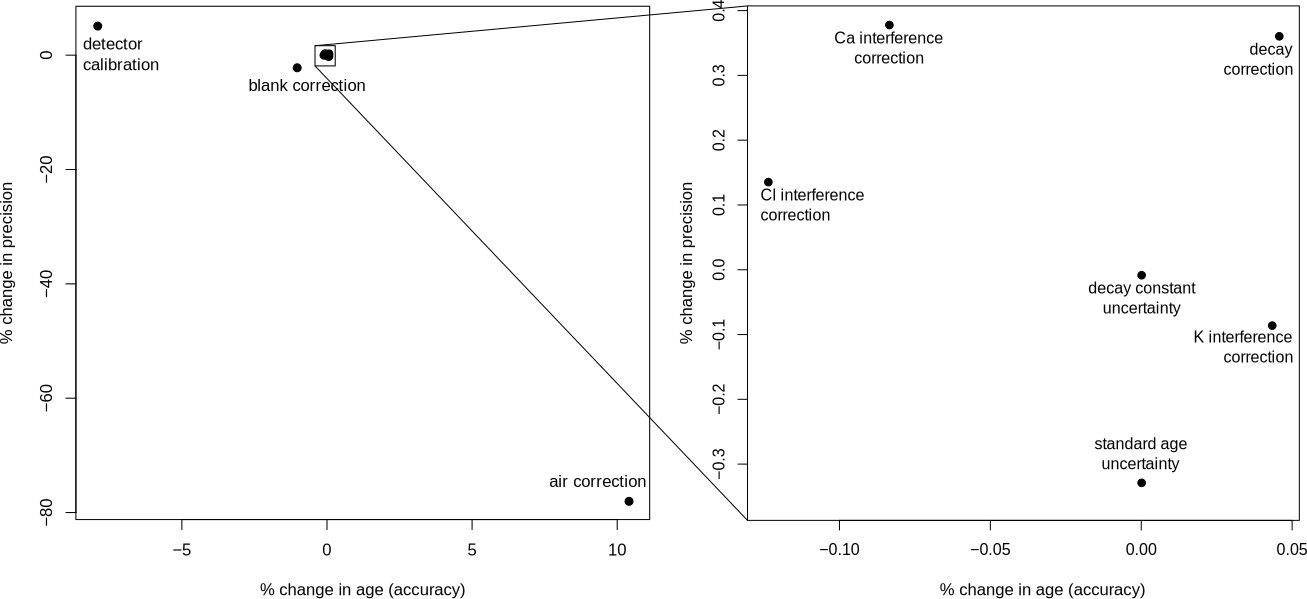
\includegraphics[width=\textwidth]{accuracyVSprecision.pdf}
  \caption{Sensitivity analysis for a single total fusion analysis of
    a $527 \pm 2 ka (1\sigma)$ sanidine crystal, showing the effect of
    omitting specific steps in the data processing chain on the
    accuracy (horizontal axis) and precision (vertical axis) of the
    results. The white square in the right panel shows the best age
    estimate using all corrections.}
  \label{fig:accuracyVSprecision}
\end{figure}

\bibliographystyle{/home/pvermees/Dropbox/abbrvplainnat}
\bibliography{/home/pvermees/Dropbox/biblio}

\end{document}
